

\section{To leave or to remain in the lattice}\label{sec:lattice_O}

Many authors, especially in recent years, have taken interest in answering the following question for various oxygen evolution electrocatalysts, both for alkaline and acidic media:
\begin{question}
During oxygen evolution, is lattice oxygen from the electrode material incorporated in the \ch{O2} produced? \label{q:lattice}
\end{question}
The question is, in other words, whether a material shows ``lattice oxygen evolution''. This is a slightly different phrase from ``lattice oxygen exchange'' more often used in the literature since both imply that oxygen is coming out of the material, but the former does not necessarily imply that new oxygen is going into the material.

\begin{figure}[b!]
	\centering
	\includegraphics[width=1\textwidth]{04_Oxygen/fig/Grimaud_and_Geiger.png}
	\caption{Examples of reported studies probing lattice oxygen evolution. The result of the isotope labeling experiment and the proposed mechanism is shown. \textbf{(a)}, Some perovskite materials including \ch{La_{0.5}Sr_{0.5}CoO_{3-$\delta$}} show lattice oxygen evolution during OER in 0.1 M \ch{KOH}. Taken from ref. \citen{Grimaud2017}. \textbf{(b)} Hydrous \ch{IrO$_x$} formed by potential cycling \ch{Ir^{18}O2} in labeled electrolyte shows lattice oxygen evolution in 0.1 M \ch{HClO4}. Taken from ref. \citen{Geiger2018}}
	\label{fig:GG}
\end{figure}

The answer to Question \ref{q:lattice}, which can be probed by isotope labeling experiments as described below, is often claimed to have profound mechanistic implications. Figure \ref{fig:GG} shows two examples from recent works by Grimaud et al\cite{Grimaud2017} in alkaline OER and from Geiger et al\cite{Geiger2018} in acid OER. Both observe evidence of an ``isotope signal'' for some of the materials studied, whereby the oxygen evolved contains an isotopic label incorporated into the catalyst, implying an affirmative answer to Question \ref{q:lattice}. The authors take the further step (which I will claim in this Thesis requires further nuance) of concluding that lattice oxygen \textit{exchange} is an important part of the OER mechanism for these materials. They propose the mechanisms shown.

To better test for and interpret lattice oxygen evolution, researchers should agree on a working definition of lattice oxygen (to distinguish from, e.g. surface-adsorbed oxygen and intercalated water). This is, to the best of my knowledge, broadly lacking. For this Thesis, I use the following definition:

\begin{definition}
	Lattice oxygen is oxygen with oxygen-metal bonds which does not reduce to water or exchange spontaneously with oxygen in the electrolyte at any potential anodic of the open-circuit potential of the material. 
	 \label{d:lattice}
\end{definition}

This definition is one motivated by practicality: lattice oxygen is, in other words, the oxygen for which Question \ref{q:lattice} can be answered by isotope-labeling studies. Any oxygen that exchanges spontaneously with the electrolyte will be lost between when the sample touches the electrolyte and when oxygen is produced. This definition of lattice oxygen excludes, for example, \ch{$*$ OH} on a Pt surface, which has a potential-dependent coverage and is thus in equilibrium with \ch{H2O} over a range of potentials. For the rutile \ch{RuO2} (110) surface, the oxygen bridging two ruthenium atoms is strongly bound with two metal bonds and at most one proton at and above 0.7 V vs RHE\cite{Rao2017a}, and so would probably be counted as lattice oxygen (the open-circuit potential in 0.1 M \ch{HClO4} after air exposure is approximately 0.9 V vs RHE); whereas oxygen adsorbed at the CUS site is in equilibrium with \ch{H2O} up to about 1.2 V vs RHE\cite{Rao2017a}, and so would not count as lattice oxygen.

An argument could be made that surface-bound oxygen, even if it fits Definition \ref{d:lattice}, is not really lattice oxygen, and that lattice oxygen should only include oxygen below the surface monolayer. This definition of lattice oxygen would make the mere detection of an isotope signal insufficient to answer Question \ref{q:lattice}, since the isotope signal could be coming from the surface monolayer. To prove that subsurface lattice oxygen is evolved during OER, more than one monolayer-equivalent of isotope signal would have to be detected.

\begin{figure}[t!]
	\centering
	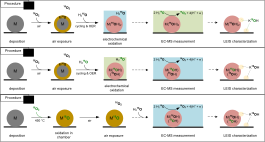
\includegraphics[width=1\textwidth]{04_Oxygen/fig/Strategies_diagram.png}
	\caption{Three strategies for isotope-labeling experiments intended to detect lattice oxygen involvement in the OER, diagrammed for the case of vacuum-synthesized \ch{NiFe} nanoparticles. Taken from Paper \ref{Roy2018}. \textbf{(a)} Strategy A involves mass spectrometric detection of evolved \ch{O2} (EC-MS step) for an unlabeled catalyst in labeled electrolyte. \textbf{(b)} Strategy B involves electrochemical labeling of an OER catalyst followed by EC-MS in an un-labeled electrolyte. \textbf{(b)} Strategy C involves direct preparation (here by annealing in \ch{^{18}O2}) of a labeled electrocatalyst followed by EC-MS in an un-labeled electrolyte.}
	\label{fig:strategies}
\end{figure}


\begin{table}
	
	\begin{tabular}{p{3cm}|p{3cm}|p{2cm}|p{2cm}|p{2cm}|p{2cm}|p{2cm}}
		Electrocatalyst & Preparation & Labeling & Electrolyte & Experiment & Result & Citation \\
		\hline
		Pt & On DEMS membrane, oxidized in 98\% \ch{H2^{18}O} & $\le$ 98\% \ch{^{18}O} & Natural 0.5 M \ch{H2SO4} or 1.0 M KOH & LSV, DEMS & no excess \ch{^{18}O} evolved & Willsau, 1985\cite{Willsau1985}\\
		\hline
		Ru and \ch{RuO2}& Sputtered onto Teflon DEMS membrane& Natural & 0.5 M \ch{H2SO4} in 90\% \ch{H2^{18}O} & CVs, DEMS & some excess \ch{^{16}O} evolved &  Wohlfahrt-Mehrens, 1987\cite{Wohlfahrt-Mehrens1987} \\ 
		\hline
		Hydrous \ch{IrO_x} & Thermal decomposition of \ch{HIrCl6} on Ti & Natural & 1 M \ch{HClO4} in 10\% \ch{H2^{18}O} & CVs, DEMS \& chip EC-MS & $>$ 1 ML excess \ch{^{16}O} evolved & Fierro, 2007\cite{Fierro2007}; rep. in Roy, 2018 \\
		\hline
		nanocrystalline \ch{RuO2} and \ch{Ru_{0.9}Ni_{0.1}O_{2-$\delta$}} & (co-)deposition on Ti mesh and annealing & Natural & 0.1 M \ch{HClO4} in 98\% \ch{H2^{18}O}& CVs, DEMS & Some excess \ch{^{18}O} evolved at high $\eta$ & Macounova, 2009\cite{Macounova2009}\\
		\hline
		Molecular Cobaltate Clusters &Electrodeposition of 0.5 mM \ch{Co^{2+}} in labeled phosphate & $\approx$ 87\% \ch{^{18}O} & Natural phosphate buffer& CP, integral headspace& 7-15\% of \ch{^{18}O} loading evolved& Surendranath, 2010\cite{Surendranath2010}\\
		\hline
		\ch{AuO_x} & Au oxidized at 2.0 V in 98\% \ch{H2^{18}O}& $\le$ 98\% \ch{^{18}O}& Natural 1 M \ch{HClO4}& LSV, OLEMS & $\approx$ 1 ML \ch{^{18}O2} evolved & Diaz-Morales, 2013\cite{Diaz-Morales2013} \\ 
		\hline
		polycrystalline, (110), (100), (101), and (111) \ch{RuO2} & oxidized in 98\% \ch{H2^{18}O} & $\le$ 98\% \ch{^{18}O} & Natural 0.1 M \ch{KOH} or 0.1 M \ch{H2SO4} & CVs, OLEMS & Little to no excess \ch{^{18}O} evolved & Stoerzinger, 2017\cite{Stoerzinger2017}\\
		\hline
		Spinel \ch{Co3O4} & as-received & Natural & 0.5 M KOH in 10\% \ch{H2^{18}O} & CVs, DEMS & 34\% ML excess \ch{^{16}O} evolved & Amin, 2017 \cite{Amin2017} \\
		\hline
		Spinel \ch{Co3O4} & electrochemically cycled in 10\% \ch{H2^{18}O} & $\le10\%$ \ch{^{18}O} & Natural 0.5 M KOH & CVs, DEMS & 12\% ML excess \ch{^{18}O} evolved & Amin, 2017 \cite{Amin2017} \\
		\hline
		\ch{LaCoO3} & solid-state synthesis, oxidized in 98\% \ch{H2^{18}O}  & $\le$ 98\% \ch{^{18}O} & Natural 0.1 M KOH & CVs, OLEMS & little to no excess \ch{^{18}O} evolved & Grimaud, 2017\cite{Grimaud2017}\\
		\hline
		\ch{La_{0.5}Sr_{0.5}CoO_{3-$\delta$}}& solid-state synthesis, oxidized in 98\% \ch{H2^{18}O}  & $\le$ 98\% \ch{^{18}O} & Natural 0.1 M KOH & CVs, OLEMS & Some excess \ch{^{18}O} evolved & Grimaud, 2017\cite{Grimaud2017}\\
		\hline
		\ch{Pr_{0.5}Ba_{0.5}CoO_{3-$\delta$}}& solid-state synthesis, oxidized in 98\% \ch{H2^{18}O}  & $\le$ 98\% \ch{^{18}O} & Natural 0.1 M KOH & CVs, OLEMS & Some excess \ch{^{18}O} evolved & Grimaud, 2017\cite{Grimaud2017}\\
		\hline
		\ch{SrCoO_{3-$\delta$}}	& solid-state synthesis, oxidized in 98\% \ch{H2^{18}O}  & $\le$ 98\% \ch{^{18}O} & Natural 0.1 M KOH & CVs, OLEMS & Some excess \ch{^{18}O} evolved & Grimaud, 2017\cite{Grimaud2017}\\
		\hline
		\ch{Ni_{0.75}Fe_{0.25}O_xH_y} film & electrodeposition & Natural & 0.1 M KOH in 97\% \ch{H2^{18}O} & CVs, chip EC-MS  & $\ll$0.1\% lattice O evolution & Roy, 2018\cite{Roy2018a} (Paper \ref{Roy2018})\\
		\hline
		\ch{Ni_{0.75}Fe_{0.25}O_xH_y}, 7 nm nanoparticles & cluster source, electrochem. oxidation & Natural & 0.1 M KOH in 97\% \ch{H2^{18}O} & CVs, chip EC-MS, ISS  & $\ll$0.1\% lattice O evolution & Roy, 2018\cite{Roy2018a} (Paper \ref{Roy2018})\\ 
		\hline
		\ch{Ni_{0.75}Fe_{0.25}O_xH_y}, 7 nm nanoparticles & cluster source, electrochem. oxidation in 97\% \ch{H2^{18}O} & Estimated 50\% \ch{H2^{18}O} & Natural 0.1 M KOH & CVs, chip EC-MS, ISS & $\ll$0.1\% lattice O evolution & Roy, 2018\cite{Roy2018a} (Paper \ref{Roy2018})\\ 
		\hline
		\ch{Ni_{0.75}Fe_{0.25}O_xH_y}, 7 nm nanoparticles & cluster source, thermal oxidation in \ch{^{18}O2} & Estimated 50\% \ch{H2^{18}O} & Natural 0.1 M KOH & CVs, chip EC-MS, ISS & $\ll$0.1\% lattice O evolution & Roy, 2018\cite{Roy2018a} (Paper \ref{Roy2018})\\ 	
		\hline
		Rutile \ch{IrO2} & Reactive sputter deposition with 99\% \ch{^{18}O2}& $\approx$ 99\% \ch{^{18}O} & Natural 0.1 M \ch{HClO4} & CP, OLEMS & little to no \ch{^{18}O} evolved& Geiger, 2018\cite{Geiger2018}\\
		\hline
		Hydrous \ch{IrO_x} & Potential cycling of sputtered \ch{Ir^{18}O2} film in 97\% \ch{H2^{18}O} & $\approx$ 97\% \ch{^{18}O}& Natural 0.1 M \ch{HClO4} & CP, OLEMS & some \ch{^{18}O} evolved& Geiger, 2018\cite{Geiger2018}\\
		\hline
	\end{tabular}
	\caption{Isotope-labeling experiments in the water oxidation electrocatalysis literature}\label{tab:lattice_lit}
\end{table}


The examples in Figure \ref{fig:GG} are but two of many studies seeking to answer Question \ref{q:lattice}. Table \ref{tab:lattice_lit} shows a more comprehensive list. The studies go all the way back to some of the earliest DEMS studies in the 1980's but have accelerated in the past couple years. The experimental methods (catalyst preparation, isotope labeling technique, electrolyte, and isotope exchange experiment measurement technique) are included to aid comparison of the various studies. One clear characteristic of this compilation is that there is no convergence yet in the literature on the best way to conduct these lattice exchange experiments.

The studies are approximately evenly split between DEMS or OLEMS for measuring the evolved oxygen isotopes. Most studies examine the oxygen evolved during potential sweeps (liniear sweep voltammatry, LSV) or cyclic voltammatry (CV), whereas only a few use constant-current measurements (CP). This is a problem because the redox changes during a potential sweep can destabilize electrode materials\cite{Kasian2016, Cherevko2016}, perhaps giving an isotope signal that would not be present in steady-state OER. Of those that measure a lattice oxygen evolution signal, some attempt to quantify the signal in terms of the total or surface oxygen loading of the catalyst\cite{Fierro2007, Surendranath2010, Diaz-Morales2013, Amin2017} whereas many observe an isotope signal but do not quantify it\cite{Wohlfahrt-Mehrens1987, Grimaud2017, Geiger2018}. 

The most pronounced difference between the experiments is in how the catalyst and electrolyte are isotope labeled. Broadly, there are three strategies:

\begin{itemize}
	\item A. The catalyst is prepared without any labeled oxygen. The lattice oxygen is thus 0.2\% \ch{^{18}O}. Oxygen evolution is then measured in labeled electrolyte with an increased \ch{^{18}O} concentration\cite{Wohlfahrt-Mehrens1987, Fierro2007, Macounova2009, Amin2017, Roy2018a}.
	
	\item B. The catalyst is originally prepared with the natural isotopic ratio, but then it is used for oxygen evolution in a labeled electrolyte. If the OER mechanism involves an exchange between the lattice oxygen and the electrolyte, this will result in labeling of the electrocatalyst with a \ch{^{18}O} concentration in the active lattice sites up to that of the electrolyte. This electrochemically labeled catalyst is then transferred to un-labeled electrolyte, and the isotopic composition of the evolved oxygen is measured.\cite{Willsau1985, Diaz-Morales2013, Stoerzinger2017a, Amin2017, Grimaud2017, Roy2018a}.
	
	\item C. The final strategy is to prepare the catalyst from the start with labeled oxygen, and then measure the isotopic composition of the the \ch{O2} evolved in labeled oxygen. Techniques to synthesize a labeled catalyst include electrodeposition in labeled electrolyte\cite{Surendranath2010}, heating a metal precursor in a \ch{^{18}O2} atmosphere\cite{Roy2018a}, and reactive sputtering with \ch{^{18}O2} in the sputtering plasma\cite{Geiger2018}.
\end{itemize}

These three strategies are illustrated schematically for the case of mass-selected nanoparticles in Figure \ref{fig:strategies}, taken from Paper \ref{Roy2018}. The coming Subsection motivates and describes the isotope labeling studies in that paper.

All of the experiments described in this Section are somewhat tedious to describe, especially because I have gradually been identifying mistakes in their procedures and learning to do them better. The Subsections of this Section may help in understanding many of the techniques used in literature, especially our own Paper \ref{Roy2018}, but a reader who is pressed for time may wish to skip to Section \ref{sec:dissolving}, which shows what I've come to think is the ``correct way'' to do isotope-labeling experiments. 

\subsection{Determining the TOF in NiFe nanoparticles}

As described in Subsection \ref{subsec:NiFe}, our group prepared a model system of vacuum-synthesized, mass-selected \ch{Ni_{0.75}Fe_{0.25}} nanoparticles in order to determine the turn-over frequency (TOF) of nickel-iron based electrodes for water oxidation in alkaline media. The primary motivation for the isotope-labeling experiments in this project was actually not to probe lattice oxygen reactivity, but instead to inform our estimate of the number of active sites for the TOF calculation, as explained below. The full story is in Paper \ref{Roy2018}. 

\begin{figure}[h!]
	\centering
	\includegraphics[width=1\textwidth]{04_Oxygen/fig/NiFe_redox_vs_surface.png}
	\caption{Activity and redox feature of \ch{NiFeO_xH_y} nanoparticles in 1.0 M KOH. \textbf{(a)}, Turn-over frequencies using three different assumptions about the number of active sites, as a function of particle size. \textbf{(b)}, Cyclic voltammagrams of all samples used for the TOF measurements, zoomed in on the redox feature. \textbf{(c)}, The number of electrons transfered in this redox feature, normalized to the calculated number of surface atoms, as a function of particle size. Taken from Paper \ref{Roy2018}. (a) is from the main text and (b) and (c) are from the SI.}
	\label{fig:redox_vs_surf}
\end{figure}

The activity of nanoparticles for a given (electro)catalytic reaction is influenced by the nanoparticle size\cite{Mistry2016b}. In general, the mass-normalized activity increases with smaller nanoparticle size, as the surface area to volume ratio of a particle increases with decreasing diameter. However, this is not always the case. If, for example, the reaction is most facile on a specific type of surface site (for example, if terraces are more active than edges), then there can be an optimum in nanoparticle size. This appears to be the case, for example, in \ch{CO2} reduction to hydrocarbons on copper nanoparticles\cite{Reske2014} and oxygen reduction on platinum nanoparticles\cite{Hernandez-Fernandez2014}. Alternately, if the bulk of a material is active for a reaction, as has been suggested for NiFe-based OER catalysts\cite{Batchellor2015, Doyle2017}, then the mass-normalized activity would not vary with nanoparticle size.

As mentioned in Subsection \ref{subsec:NiFe}, the cluster source synthesis enables us to know the exact mass and surface loading of each sample. Figure \ref{fig:redox_vs_surf}a shows the turn-over frequency at 1.53 V as a function of nanoparticle size vs RHE calculated with three different assumptions about the number of active sites: TOF$_{\text{bulk}}$ assumes all metal atoms are active, TOF$_{\text{surface}}$ assumes metal atoms on the outer surface of the nanoparticle are active, and TOF$_{\text{redox}}$ assumes one active site per electron transfered during the \ch{Ni^{2+}/Ni^{3+/4+}} redox couple just before the onset of OER. This redox couple is shown for all of the samples in the CV's in Figure \ref{fig:redox_vs_surf}b.

Since TOF$_{\text{bulk}}$ (which is proportional to the mass-normalized activity) does indeed decrease with increasing nanoparticle size, we conclude that the bulk of these nanoparticles do not participate in the oxygen evolution reaction. On the other hand, the TOF$_{\text{surface}}$ and TOF$_{\text{redox}}$ do not show clear trends with nanoparticle size. This is consistent with each surface atom being an active site, or with each electron transferred during the redox wave representing an active site. For the electrodeposited NiFe LDH (also described in Subsection \ref{subsec:NiFe}), the exact loading was unknown and so only TOF$_{\text{redox}}$ is shown. This is lower than TOF$_{\text{redox}}$ for the nanoparticles, indicating either that the number of electrons transferred in the redox feature is not the best way to measure the number of active sites, or that the activity of the active sites differ for these two differently synthesized materials.

Figure \ref{fig:redox_vs_surf}c shows the number of redox electrons per Ni atom (black, left y-axis) and per surface Ni atom (red, right y-axis). The latter is equal to the ratio between TOF$_{\text{surface}}$ and TOF$_{\text{redox}}$. For the smallest nanoparticles, the entire nanoparticle appears to be redox active, with approximately one redox electron transferred per nickel atom in the sample, whereas for the larger nanoparticles, there are fewer than 1 electron transferred per nickel atom, indicating that the particles have a redox-inactive core. There are three to five electrons transferred per surface Ni atom, indicating that the redox feature penetrates below the outer surface of the nanoparticles. The question is then whether the redox-accessible portion of the nanoparticle is also OER active. This is illustrated in Figure \ref{fig:NP_diagram}.

\begin{figure}[h!]
	\centering
	\includegraphics[width=0.8\textwidth]{04_Oxygen/fig/NP_diagram.png}
	\caption{Two competing models of the nickel redox feature and oxygen evolution in NiFe nanoparticles. \textbf{Left}, The redox-active near-surface region is permeable to \ch{OH-} and \ch{O2}, and contributes to the OER. \textbf{Right}, The redox-active near-surface region is only accessible by proton shuttling and does not contribute to OER. The diagram on the far left of a proposed layered structure for the redox-permeable NiFeOOH region is from Friebel, 2015, ref. \citen{Friebel2015}.}
	\label{fig:NP_diagram}
\end{figure}

The question of whether the redox-active near-surface region contributes to OER is related to the question of which species carries the charge in and out of this region during the redox transition. If it is \ch{OH-}, then it is reasonable to believe that \ch{H2O} and \ch{O2} can also move through the near-surface region, and that the near-surface region can contribute to the OER, which in alkaline electrolyte can be written
\begin{equation}
\ch{4 OH- -> O2 + 2 H2O + 4 e-}\,.\label{rxn:OER_alkaline}
\end{equation}
Unfortunately, the transport mechanism involved in the nickel redox feature is still not known\cite{Dionigi2016b}. It is often written by the nominal reaction 
\begin{equation}
\ch{Ni(OH)2 <-> NiOOH + (H+ + e- )}\,,\label{rxn:Ni_redox}
\end{equation}
but in addition to protons, hydroxide and solvated cations have all been suggested as possible charge carriers\cite{WehrensDijksma2006}.

We therefore sought to answer the question by another means. We reasoned that, if the redox-active subsurface region participated in the oxygen evolution reaction, then the \ch{H2O} and/or \ch{OH-} originally in that region would be oxidized to \ch{O2} which we could differentiate from oxidation of the bulk electrolyte by isotope labeling. We performed the three isotope-labeling procedures described in Figure \ref{fig:strategies} on mass-selected 7nm NiFe nanoparticles:


\begin{figure}[p]
	\centering
	\includegraphics[height=0.8\textheight]{04_Oxygen/fig/Roy2018_raw_results.png}
	\caption{EC-MS results for isotope experiments on \textbf{(a-c)} NiFe NP’s (a, b, and c correspond to procedures A, B, and C in Figure \ref{fig:strategies}); and \textbf{(d)} an electrodeposited NiFe thin film and \textbf{(e)} an \ch{IrO_x} thin film produced by thermal decomposition of \ch{HIrCl6} in air, by procedure A. The signal for \ch{O2} produced in the largest portion by oxidation of the electrolyte (m/z=36 for procedure A and m/z=32 for procedures B and C) is plotted on the right y-axis, and the other \ch{O2} isotope(s) on the left y-axis. m/z=32 is omitted as a minority isotope since it is dominated by the background due to residual natural \ch{O2}. (f) The excess minority isotope (\ch{^{16}O} for procedure A and \ch{^{18}O} for procedures B and C) is quantified and normalized to (solid bars, left y-axis) the number of surface atoms in the catalyst or to (hashed bars, right y-axis) the total \ch{O2} evolved during the part of the experiment shown here. From the SI of Paper \ref{Roy2018}}
	\label{fig:Roy2018_raw_results}
\end{figure}

For procedure A, the as-synthesized nanoparticles were cycled between 0.5 V and 1.6 V vs RHE in un-labeled electrolyte, to form the hydrated redox-accessible near-surface region implied by Figure \ref{fig:redox_vs_surf}c. The sample was then transferred to the EC-MS setup, where the cell was filled with labeled electrolyte (0.1 M KOH in 97\% \ch{H2^{18}O}), and the potential was cycled up to where oxygen was evolved (1.55 V vs RHE). The advantage to procedure A is that there is no doubt about the initial isotopic composition of the oxygen in the catalyst, as the electrode has only been exposed to natural oxygen. The disadvantage is that the \ch{^{16}O} impurity in the labeled electrolyte limits the sensitivity. 

For procedure B, the as-synthesized nanoparticles were cycled between 0.5 and 1.6 V vs RHE in labeled electrolyte. A disadvantage here is that there is inevitably less than perfect control over the isotopic composition of the electrocatalyst, since it might interact with air after being taken out of the vacuum chamber and before being placed in labeled electrolyte. We actually tried to minimize this by having a pipette with labeled electrolyte ready at the load-lock, and could bring down the time in air to 15 seconds, but in 15 seconds on the order 0f 10$^7$ \ch{^{16}O2} molecules will have hit each surface site and had a chance to react \cite{Concepts2003}. We expect, as a worst case, that the oxygen in the labeled catalyst consists of 50\% \ch{^{18}O}, due to formation of \ch{M^{16}O}, with M=\ch{Ni_{0.75}Fe_{0.25}}, when exposed to air and subsequent formation of \ch{M(^{16}OH)(^{18}OH)} when cycled in labeled electrolyte. This is indicated in Figure \ref{fig:strategies}.

For procedure C, the as-synthesized nanoparticles were left in the vacuum chamber, where \ch{^{18}O2} was dosed and the sample was heated to 450$^\circ$C. The nanoparticles were thus already oxidized when taken out into air, and presumably retained a high degree of labeled isotopic purity and the nominal \ch{M^{18}O} formula. However, the sample was then put directly into the EC-MS setup with un-labeled electrolyte, where the nanoparticles likely hydrated to \ch{M(^{18}OH)(^{16}OH)} as illustrated. In hindsight, it would have been better to cycle the particles in labeled electrolyte prior to EC-MS testing to achieve a nominal \ch{M(^{18}OH)2} formula.

In addition to the NiFe nanoparticles, we also tested an electrodeposited NiFe oxyhydroxide film (described in subsection \ref{subsec:NiFe}) in the same electorlyte, and an \ch{IrO_x} material produced by thermal decomposition of \ch{HIrCl6}. The latter material was produced by dropcasting a solution of 5 mM \ch{HIrCl6} on a titanium stub and annealing in air at 500$^\circ$C for two hours. This is the same material tested for lattice exchange in Fierro et al, 2007, ref. \citen{Fierro2007}. In that study, the authors saw a significant amount of lattice oxygen evolution as an excess \ch{^{16}O} signal during the first cyclic voltammagrams in \ch{^{18}O}-labeled electrolyte (see Table \ref{tab:lattice_lit}). Both the NiFe oxyhydroxide electrodeposited film and the thermal decomposition \ch{IrO_x} samples were tested according to Procedure a: They were prepared with the natural isotope ratio, and tested for lattice exchange in labeled electrolyte. The NiFe film was tested in 0.1 M KOH in 97\% \ch{H2^{18}O} like the NiFe nanoparticles. The \ch{IrO_x} was tested in 1.0 M \ch{HClO4} in 97\% \ch{H2^{18}O}. The higher concentration of \ch{HClO4} meant that the final isotopic purity of the electrolyte was lower.

The raw EC-MS results for these five isotope-labeling experiments (NP's procedure A-C, NiFe film and \ch{IrO_x} procedure A) are shown in Figure \ref{fig:Roy2018_raw_results}a-e. 

Here, a quick note on this plotting form: in this type of isotope labeling experiments, a ``positive'' result is an isotope signal originating from the electrocatalyst, namely a (transient) isotopic composition of the evolved \ch{O2} that cannot be explained by the composition of the electrolyte. A ``negative'' result, on the other hand, is one in which the isotopic composition of the evolved \ch{O2} always reflects the isotopic composition of the electrolyte. It therefore makes sense to plot the results in a way where deviations of the measured \ch{O2} signal and the expected \ch{O2} from oxidation of the electrolyte are clearly visible. After trying a few different plotting strategies, our group thinks that the best way to do so, without hiding any information, is to co-plot the MS signals, scaled according to the expected ratio. This can be done by multiplying one of the signals by the expected ratio, or by using two y-axes scaled according to the expected ratio. The latter technique is used in Figure \ref{fig:Roy2018_raw_results}a-e. In each case, the ``expected ratio'' was taken to be the background-corrected steady-state ratio during a constant-current OER measurement (0.5 mA/cm$^2$ for 10 minutes) taken right after these cycles. In this constant-current period, the total amount of \ch{O2} evolved was much greater than the amount of oxygen in the catalyst, ensuring that the steady-state ratio reflected the isotopic concentration of the bulk electrolyte.

When plotted this way, it is immediately clear that there is a very small amount of excess \ch{^{18}O} evolved in procedure B (Figure \ref{fig:Roy2018_raw_results}b) in the form of \ch{^{18}O2} (m/z=36) and \ch{^{18}O^{16}O} (m/z=34), a much larger amount of excess \ch{^{16}O} evolved from \ch{IrO_x} (\ref{fig:Roy2018_raw_results}e) in the form of \ch{^{18}O^{16}O}, and little to no isotope signal in any of the other samples.

The astute reader may have noticed a rather important experimental mistake: each experiment starts with an anodic scan from OCP, but for the NiFe nanoparticles in both procedures A (Figure \ref{fig:Roy2018_raw_results}a) and C (Figure \ref{fig:Roy2018_raw_results}c), the first cycle does is not anodic enough to produce a significant \ch{O2} signal, and the sample is cycled through the Ni redox couple before a significant amount of \ch{O2} is evolved. If oxygenated species are transferred or mobile during that redox reaction, then the labeled intercallated \ch{OH-} or \ch{O2} might escape to the bulk electrolyte before it can be oxidized to \ch{O2} and detected. We were aware of this mistake while preparing the manuscript, but did not get a chance to repeat these experiments, which were quite challenging for two reasons: (1) The cluster source synthesis was expensive and demanding, and (2) The membrane chips used in the EC-MS experiments at the time were not alkaline-resistant, and so chips would often breach during the measurement. So, after much frustration, we decided to use this data. We concluded, however, that it did not influence the interpretation of the results, for the following reasons: (1) We figured that at least some of the \ch{O} species, such as those bound to nickel in \ch{OH} groups, would stay put during the redox reaction, and (2) The results for procedures A and C were broadly consistent with the results for procedure B (Figure \ref{fig:Roy2018_raw_results}b) and for the electrodeposited film (Figure \ref{fig:Roy2018_raw_results}c), where the anodic potential of the first scan was high enough to give a significant oxygen signal. 

In hindsight, this mistake is part of the simpler and more general mistake of using potential scans rather than constant-potential or (even better) constant-current experiments, since, in general, it is best to hold as much constant as possible when studying a transient phenomenon. In this case, it is best to hold the total \ch{O2} production rate constant when studying potentially transient changes in its isotopic composition.

Figure \ref{fig:Roy2018_raw_results}f shows a quantitative comparison of the five isotope-exchange experiments from Figure \ref{fig:Roy2018_raw_results}a-e. The excess lattice oxygen (\ch{^{16}O} for procedure A and \ch{^{18}O} for procedures B and C) is calibrated and normalized to either the number of surface sites (i.e., monolayers, solid bars, left y-axis) or to the total amount of \ch{O2} evolved (right y-axis). In the case of the \ch{IrO_x} catalyst, a significant portion ($\approx$ 6\%) of the \ch{O2} contained ''unexpected'' \ch{^{16}O}, indicating that it came from the lattice. For all of the NiFe samples, the portion of the evolved \ch{O2} containing \ch{O} from the lattice was under 0.5\%, with the apparent highest amount coming from the film and the nanoparticles tested by procedure A. Procedure A has the highest expected amount of \ch{^{16}O^{18}O} because the purity of the labeled electrolyte ($\le$ 97\% \ch{H2^{18}O}) is less than than the purity of the un-labeled electrolyte ($\approx$ 99.8\% \ch{H2^{16}O}). This indicates that the the apparent portion of evolved \ch{O2} containing lattice O when analyzed by this method is related to the noise level of the m/z=34 signal, i.e., that it doesn't necessarily represent real lattice \ch{O} evolution, which could be zero. The amount of lattice \ch{O} evolved, when normalized to the number of surface sites, is $\approx$ 2 monolayers for the \ch{IrO_x} catalyst and $\le$ 2\% of a monolayer for all NiFe samples. 

We concluded therefore, that only the outer surface of the nanoparticles are active, implying that the turn-over frequency closest to the truth is TOF$_{\text{surface}}$, which for the 5.4 nm nanoparticles is $\approx$ 6 s$^{-1}$. This is a record for OER in alkaline electrolyte, as shown in Figure \ref{fig:alkaline_TOF} at the start of this Chapter.

\begin{figure}[p]
	\centering
	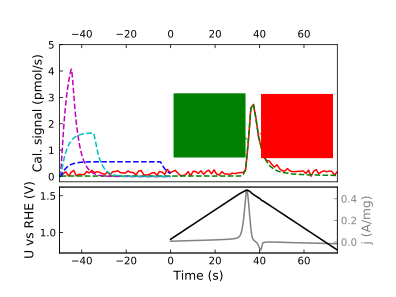
\includegraphics[height=0.8\textheight]{04_Oxygen/fig/NiFe_ECMS_resuls_model.png}
	\caption{\textbf{(a-c)} Analysis of EC-MS results and \textbf{(d-f)} ISS spectra of the samples as-prepared and post-OER for procedures A (a and d), B (b and e), and C (c and f). The experimental procedures are illustrated in Figure \ref{fig:strategies} and the raw EC-MS data is shown in Figure \ref{fig:Roy2018_raw_results}. The modeled signal for 1\% exchange of lattice oxygen should be compared to the \textit{difference} between the expected and measured \ch{^{16}O^{18}O} signal. Procedure A is from the main text and Procedures B and C are from the SI of Paper \ref{Roy2018}}
	\label{fig:Roy2018_model}
\end{figure}

Even if the experimental mistake mentioned above weakens the conclusion that the redox-active near-surface region does not participate in the OER, it does not invalidate these experiments as evidence for the other conclusion of the isotope-labeling experiments: Lattice oxygen is not exchanged during the oxygen-evolution reaction. This relies on Definition \ref{d:lattice} of lattice oxygen, which excludes oxygen that would be exchanged in the \ch{Ni^{2+}/Ni^{3+}} redox feature.

To illustrate the sensitivity of the experiments for lattice oxygen evolution, if it occurred, we plotted the data in another way. The majority isotope from electrolyte oxidation (\ch{^{18}O2} for procedure A, \ch{^{16}O2} for procedures B and C) is scaled down according to the isotopic composition of the electrolyte and plotted on the same axes as the other two \ch{O2} isotopic signals, as the ``expected'' \ch{^{16}O^{18}O} signal. The first scan with significant oxygen evolution is shown for each sample.  On the same axes, we plot the expected excess \ch{^{16}O^{18}O} signal if just 1\% of the lattice \ch{O} were to come out as \ch{O2}. The area of this signal (in pmol) is based on the known metal loading and the nominal formula in Figure \ref{fig:strategies}. The shape is based on the mass transport model in Paper \ref{Trimarco2018}. This modeled signal should be compared to the \textit{difference} between the measured and expected \ch{^{16}O^{18}O} signals. In all cases, it is clear from the difference of the measured and expected signals, and the noise levels, that much less than 1\% of the lattice \ch{O}, if any, is evolved during the first cycle.

Finally, if lattice oxygen is not exchanged during OER, that should mean that it is still present in the catalyst afterwards. To test this we did ion scattering spectroscopy (ISS, also known as low-energy ion scattering, LEIS) on the as-deposited nanoparticle samples, and again after the EC-MS experiment. The results are shown in Figure \ref{fig:Roy2018_model}d-f. The interpretation of the ISS spectra is complicated by the fact that some residual potassium, presumably in the form of KOH, is present on the surface of the sample, even after thorough rinsing with ultrapure water (procedures B and C) or labeled water (procedure A). The oxygen in this KOH thus has the isotopic composition of the electrolyte, which is the opposite of that expected in the catalyst. This likely explains the \ch{^{18}O} signal in the ISS spectrum for procedure A (Figure \ref{fig:Roy2018_model}d), whereas we explain the \ch{^{16}O} signal as lattice oxygen which has not exchanged during OER. This is supported by the fact that the \ch{^{16}O}/\ch{^{18}O} ratio increases after the sample is subject to argon sputtering in the vacuum chamber. On the other hand, the potassium signal is much lower in procedues B and C, especially after sputtering, perhaps due to the greater ease of rinsing with non-labeled water. Here, the isotope ratio converges to 1:1, which matches the nominal stoichiometry motivated in Figure \ref{fig:strategies} and the text earlier in this subsection. Together these EC-MS and ISS results make us confident that there is little to no exchange of lattice oxygen during OER in nickel-iron based catalysts for alkaline water oxidation.

\clearpage 
\subsection{A contradiction}

The attentive reader may have noticed a contradiction:

In Section \ref{sec:low_O2}, I noted that the acid-electrolyte OER activities of all \ch{RuO2} films and \ch{Ru} foams converged when normalized to the capacitance of the films, which I pointed out is consistent with an assumption that all of the surface area accessible to the electrolyte for redox and capacitive charging is also active for the oxygen evolution reaction. 

However, in Paper \ref{Roy2018}, we argue that only the outer surface of the nanoparticles is active for alkaline-electrolyte OER, even though the Ni redox feature penetrates $\approx$ 3-5 monolayers into the nanoparticles. This argument is quite central to the paper, as the conclusion that catalytic activity is confined to the outer surface of the nanoparticles is used to calculate the record TOF of 6 s$^{-1}$ at an overpotential of 300 mV. 

We motivate the argument that OER occurs only on the outer surface, and not in the redox-active near-surface region, by isotope-labeling studies that always show \ch{O2} with the same isotopic composition as that of the electrolyte. Our reasoning is that OER activity below the surface would either involve lattice oxygen evolution or oxidation of low-mobility intercalated water. We hypothesize that the redox activity below the surface is only due to proton shuttling.

This contradiction is especially troubling in consideration of the fact that unlabeled \ch{RuO2} films also do not give an isotope signal during OER in isotope-labeled electrolyte. I.e., sputtered \ch{RuO2} also gives a negative result to Strategy A in Figure \ref{fig:strategies}). This is evident, for example, in Figure \ref{fig:He_vs_O2} in the previous Section, where there is no excess \ch{^{16}O} evolution during the first cycles in \ch{^{18}O}-labeled electrolyte (i.e., the m/z=34 to m/z=36 ratio is constant throughout the experiment). Apparently, the water in the porous structure of high-surface-area \ch{Ru} and \ch{RuO2} has no trouble diffusing out of the pores before the onset of OER, unlike our assumption for NiFe oxyhydroxide.

One motivation for these differing lines of reasoning for the two materials is that the porosity is on a different scale: whereas the nanoscale domains and cavities in hydrous \ch{RuO2} are on the order of a few nanometers\cite{Yoshida2013}, the metal-metal spacing between the layers in \ch{NiFe} layered double hydride is only 0.4 to 0.8 nanometers, and the layers are interconnected by hydrogen bonds, depending on the phase\cite{Dionigi2016b}. Thus, there is more room for water and other species to diffuse in and out of amorphous \ch{RuO2}. Another is the TEM images of the NiFe nanoparticles (Paper \ref{Roy2018}, Figure 4) which indicate that they are non-porous both before and after the reaction (unfortunately, we do not have TEM images on the sputtered \ch{RuO2} films).

Nonetheless, the uncertainty evident in this contradiction, together with the imperfections mentioned above of the isotope experiments in Paper \ref{Roy2018}, mean that the conclusion of no OER activity in the redox-active near-surface region should be taken with a grain of salt. We think that these issues should motivate research into the charge transfer and mass transport processes during (near-) surface redox reactions at the oxide-electrolyte interface for oxygen evolution catalysts. A better understanding of these transport processes is essential for determining the number of sites that participate in the oxygen evolution reaction, which in turn is essential for developing catalysts with improved intrinsic activity\cite{Kibsgaard2019}. 

In defense of Paper \ref{Roy2018}, we do leave somewhat open our conclusion that only the outer surface is active, and we state clearly the assumptions that is based on. 

\subsection{Electrochemically labeled \ch{RuO2} films} \label{subsec:Ru_exchange}

As mentioned at the beginning of this Chapter, oxides of iridium and ruthenium and materials based on such oxides are the only known active and somewhat stable oxygen evolution catalysts in acidic electrolyte\cite{Reier2017, Kibsgaard2019}. The electrocatalytic mechanism of such materials has therefore been the subject of many studies, including several using isotope-labeling\cite{Wohlfahrt-Mehrens1987, Fierro2007, Macounova2009, Stoerzinger2017, Grimaud2017}. Some details of these studies are compiled in Table \ref{tab:lattice_lit}.

In Section \ref{sec:low_O2}, I described activity measurements on well-characterized sputtered \ch{RuO2} films in isotope-labeled electrolyte (0.1 M 97\% \ch{H2^{18}O}), effectively giving us procedure A of Figure \ref{fig:strategies} for free, but did not then go into detail on the possibility of lattice oxygen evolution. In contrast, in Figure \ref{fig:Roy2018_raw_results}, I showed a lattice exchange study on a poorly-characterized \ch{IrO_x} film formed by thermal decomposition of \ch{HIrCl6}, reproducing the result, first reported in reference \citen{Fierro2007}, of significant lattice oxygen evolution on that material. In this Subsection, I describe isotope-labeling experiments on the \ch{RuO2} materials described in Section \ref{sec:low_O2}. Sputtered thin films (and cluster source nanoparticles) can be thought of as a model system, in contrast to the more practical but harder-to-understand real catalysts like the thermal-decomposition \ch{IrO_x} (and electrodeposited NiFe). Compared to the previous literature, the work presented here adds the high sensitivity of the chip-based EC-MS system as well as surface isotopic characterization by ion scattering spectrometry (ISS).

Part of our motivation for studying OER in acid, in addition to the technological importance of PEM electrolyzers, was a practical consideration: The silicon membrane chips of the EC-MS setup are unstable in alkaline, but stable in acid. Thus, after a frustrating experience involving many experiments being compromised due to chips breaching in the work leading to Paper \ref{Roy2018}, we wanted to work on something (relatively) easy.

\begin{figure}[h!]
	\centering
	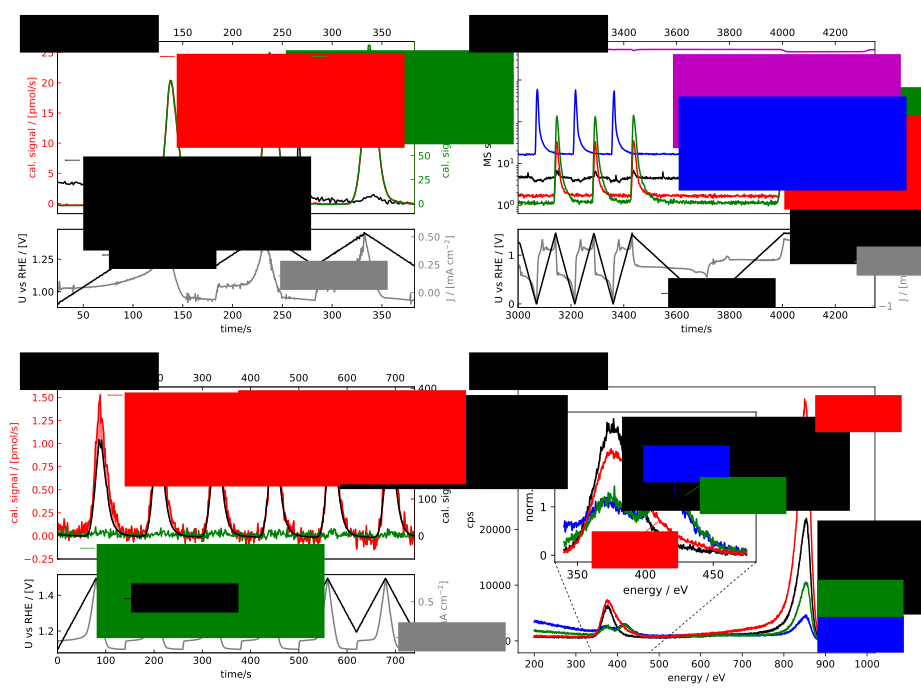
\includegraphics[width=1\textwidth]{04_Oxygen/fig/Reshma1B_lattice_O.png}
	\caption{Lattice oxygen evolution experiments on \ch{RuO2} film sputtered at room temperature with natural \ch{O2}. \textbf{(a)}, The first cyclic voltammagrams of a fresh, un-labeled sample (\ch{Ru^{16}O2}) in labeled electrolyte (0.1 M \ch{HClO4} in 97\% \ch{H2^{18}O}). The left (\ch{^{16}O^{18}O} and \ch{^{16}O2}) and right (\ch{^{18}O2}) y-axes are scaled according to the \ch{^{16}O^{18}O} to \ch{^{18}O2} measured during steady-state OER later in the experiment. \textbf{(b)}, Electrochemical labeling procedure to incorporate \ch{^{18}O} from the labeled electrolyte into an un-labeled sample. \textbf{(c)}, The first cyclic voltammagrams of an electrochemically labeled sample in unlabeled electrolyte (0.1 M \ch{HClO4} in 99.8\% \ch{H2^{16}O}). The left (\ch{^{16}O^{18}O} and \ch{^{18}O2}) and right (\ch{^{16}O2}) y-axes are scaled according to the natural \ch{^{16}O^{18}O} to \ch{H2^{16}O} ratio of 0.40\%. The area between the \ch{^{16}O^{18}O} and \ch{^{16}O2} signals thus plotted, which is approximately 50 pmol in total on the scale of the left y-axis, is highlighted. \textbf{(d)}, Ion scattering spectra of: (black) a sample that has evolved oxygen in labeled electrolyte (potential holds and cycling between 1.2 and 1.5 V vs RHE) but not brought to reducing potentials; and a sample that has been electrochemically labeled directly after loading in the vacuum chamber (blue), after 30 minutes of He sputtering (green), and after 30 minutes of Ar sputtering (red).
	}
	\label{fig:Reshma1_lattice}
\end{figure}

The isotope-labeling experimental techniques that we used at first on the \ch{RuO2} films were therefore directly taken from those described in the paper above: cyclic voltammatry of un-labeled or electrochemically labeled films, where a  ''positive'' result is a changing isotope ratio during from cycle to cycle. Figure \ref{fig:Reshma1_lattice} shows the results of such experiments on room-temperature sputtered \ch{RuO2} films. The sample was first tested according to Procedure A of Figure \ref{fig:strategies}, i.e., the isotopic ratio was observed during OER from an un-labeled sample in labeled electrolyte. The result, in Figure \ref{fig:Reshma1_lattice}a is that there is no excess \ch{^{16}O} in the evolved \ch{O2}\textit{}. The sample was then tested according to Procedure B, i.e. labeled electrochemically and then tested in un-labeled electrolyte. Procedure B can be more sensitive than Procedure A due to the high isotopic purity (99.8\% \ch{^{16}O}) of natural oxygen. 

Some authors have used steady-state OER as a labeling technique\cite{Stoerzinger2017, Grimaud2017}. This, however, only succeeds in labeling the catalyst if there is a significant amount of lattice exchange, incorporating the oxygen from the electrolyte into the catalyst. Therefore, we used ion scattering spectrometry (ISS) as a direct determination of isotope labeling. The black trace in Figure \ref{fig:Reshma1_lattice}d is an ISS spectrum of an \ch{Ru^{16}O2} film after OER in \ch{^{18}O}-labeled electrolyte (specifically, after the activity test in Figure \ref{fig:Reshma1_activities}b of the previous Section). There is a clear \ch{^{16}O} peak, centered at 375 eV, but no sign of \ch{^{18}O}, indicating that OER does not incorporate oxygen from the electrolyte into the lattice of \ch{RuO2}. This is consistent with the lack of lattice oxygen evolution that has been reported before for crystalline \ch{RuO2}\cite{Stoerzinger2017}, but the (absence of) labeling had not been directly probed. 

Since OER itself did not incorporate the oxygen from the electrolyte into the sample, to produce a labeled sample, we instead tried reducing and oxidizing the sample in labeled electrolyte. This procedure is shown in Figure \ref{fig:Reshma1_lattice}b. The sample is cycled between -0.05 V vs RHE, where hydrogen evolution takes place, and +1.4 V vs RHE, where oxygen evolution takes place. This is intended to incorporate the new isotope in the lattice according to the following nominal reactions near the surface of the electrode:
\begin{align}
\ch{Ru^{16}O2 + 4 (H+ + e- ) &-> Ru + 2 H2^{16}O}\nonumber\\
\ch{Ru + 2 H2^{18}O &-> Ru^{18}O2 + 4 (H+ + e- )}\label{rxn:Ru_labeling}
\end{align}
The sample was finally held at 1.4 V vs RHE for 5 minutes to ensure that the surface was oxidized when the sample was removed from electrolyte. 

The blue trace in Figure \ref{fig:Reshma1_lattice}d shows an ISS spectrum of a sample thus labeled. Both oxygen isotopes are clearly present. To ensure that these are not just loosely bound surface species such as adsorbed \ch{H2O} from the electrolyte and/or air, the sample was sputtered in He before taking another spectrum, shown in the green trace. The increase in the \ch{Ru} signal at $\approx$ 850 eV indicates that some surface species are indeed removed, while both oxygen isotopes remain. The presence of \ch{^{18}O} indicates that the surface of the sample was successfully labeled. However, there is still a significant amount of \ch{^{16}O}, indicating that Reactions \ref{rxn:Ru_labeling} are not carried out completely. In other words, the surface is not completely reduced during the labeling procedure. The approximately 1:1 ratio may indicate that 2 electrons are transferred rather than 4 in the (near-)surface redox processes taking place between -0.05 and 1.4 V vs RHE. Using the (110) surface to approximate the surface sites of this polycrystalline sample, the observation of 1:1 \ch{^{18}O}:\ch{^{16}O} in ISS could perhaps indicate exchange of Bridge-bound \ch{O} but not the trigonally coordinated surface \ch{O}. This is consistent with the surface species as a function of potential proposed by Rao et al, 2017, ref. \citen{Rao2017a}. In that study, using the ''crystal truncation rods'' of single-crystal x-ray diffraction, the authors show that bridge sites are fully protonated at 0.5 V vs RHE, indicating that they may exchange spontaneously with water. Any CUS-adsorbed oxygen would exchange with electrolyte, but would likely be too loosely bound for ISS observation, as it would desorb when the sample is pumped down in the vacuum chamber\cite{Over2000}. However, it should also be noted that we are by no means certain of this interpretation - it could be that both CUS and Bridge oxygen atoms are both sputtered away by He at the start of the scan, and that ISS is probing oxygen below the adsorbate layer.

To test whether the procedure in Figure \ref{fig:Reshma1_lattice} also labeled the bulk of the sample, we then sputtered the sample with argon for 30 minutes. A separate calibration experiment was done in which a 5 nm \ch{RuO2} film on Ti was sputtered through until the substrate was visible in ISS, taking a total of about 2.5 hours of Ar sputtering with all other parameters held the same. This indicates that 30 minutes of Ar sputtering removes approximately 1 nm of material. The subsequent ISS specrum, the red trace in Figure \ref{fig:Reshma1_lattice} has a much smaller \ch{^{18}O} to \ch{^{16}O} ratio, indicating that there is little to no labeling of the bulk of the material. (We don't believe the Ar sputtering to be completely uniform, so the small amount of remaining \ch{^{18}O} signal probably still comes from the surface and doesn't reflect the isotopic composition exactly 1 nm into the bulk). This sputtering, of course, was destructive to the isotope labeling of the sample, so another sample was labeled by the same procedure for an EC-MS test of lattice oxygen evolution.

Figure \ref{fig:Reshma1_lattice}c shows the oxygen evolved in unlabeled elctrolyte (0.1 M \ch{HClO4} in natural \ch{H2O}) during cyclic voltammatry of a film thus labeled. The axes are scaled according to the natural ratio such that the \ch{^{16}O^{18}O} signal (red trace, left y-axis) and \ch{^{16}O2} signal (black trace, right y-axis) would coincide exactly if all of the oxygen atoms in the evolved \ch{O2} came from the electrolyte. Compared to this baseline, there is clearly some excess \ch{^{16}O^{18}O} in the first cycles, with the isotopic ratio converging to the expected natural ratio after about six cycles. Integrating the excess \ch{^{16}O^{18}O} signal (i.e., the highlighted area in Figure \ref{fig:Reshma1_lattice}c) gives a total of 50 pmol of \ch{O} that must have originated in the lattice. Since the lattice was only 50\% labeled, this would imply that 100 pmol of lattice \ch{O} was evolved. Considering the high surface area of the room-temperature-sputtered films (Figure \ref{fig:RuO2_char}), this is only approximately 0.7\% of a monolayer. It is also only $\approx$ 0.1\% of the total \ch{O2} evolved during the first six cycles. 

Our ability to measure lattice oxygen evolution on \ch{RuO2}, in contrast to ref. \cite{Stoerzinger2017}, is due to the labeling procedure and increased sensitivity of the chip-based EC-MS technique, and is not inconsistent with their results. Our ability to quantify the evolved lattice oxygen and compare it both to the number of surface sites and to the total oxygen evolved, enable us to determine that it is negligible with respect to the OER activity. Indeed, the conclusion of the quantitative isotope-labeling studies is that the catalytically relevant OER mechanism on sputter-deposited \ch{RuO2} \textit{does not} involve lattice oxygen evolution.

As mentioned earlier in this Section, cyclic voltammatry has the disadvantage that too many things are changing at once: a potentially transient isotopic signal gets convoluted in the changing state of the catalytic surface with potential. The appeal of using scans is that, in principle, a number of potentials are quickly sampled\cite{Macounova2009}, and that the isotopic ratio can easily be compared from one scan to another\cite{Fierro2007}. However, partial reduction and re-oxidation of the (near-) surface might create unstable sites that would not be present under steady OER operation. It might also reduce out the lattice \ch{O} as water. 

\begin{figure}[t]
	\centering
	
\includegraphics[width=1\textwidth]{04_Oxygen/fig/EC_labeled_exchange.png}
	\caption{
		Constant-current water oxidation in unlabeled electrolyte on: \textbf{(a-c)} RT-sputtered \ch{RuO2}, \textbf{(d)} Ru foam, and \textbf{(e)} polycrystalline Pt, all labeled by cycling between HER and OER potentials (-0.05 and +1.4 V vs RHE for \ch{RuO2}) followed by 10 minutes of +0.5 mA/cm$^2$ geometric current density in labeled electrolyte (0.1 M \ch{HClO4} in 97\% \ch{H2^{18}O}); and \textbf{(f)} unlabeled RT-sputtered \ch{RuO2}. The noise in the mass spectrometric signal (a-e) is attributed to bubbles, and the noise in the potential measurement in f is attributed to poor contact to the alligator clip. In each case, the calibrated \ch{^{16}O^{18}O} signal (red) and \ch{^{18}O2} signal (green) are co-plotted with the \ch{^{16}O2} signal, with the latter being on the right y-axis which is scaled according to the natural \ch{^{16}O^{18}O}/\ch{^{16}O2} ratio of 0.40\%. The integrated amount of excess \ch{^{16}O^{18}O} is indicated. 
	}
	\label{fig:EC_Ru}
\end{figure}

Therefore, I also monitored the \ch{O2} evolved during constant-current measurements on electrochemically labeled \ch{RuO2} films. The films were prepared and labeled as described above (R.T. sputtered, cycled between -0.05 and +1.4 V vs RHE in labeled electrolyte). OER was then measured at 100 $\mu$A (a geometric current density of 0.5 mA/cm$^2$) for 5 minutes. The results, done in triplicate, are shown in Figure \ref{fig:EC_Ru}a-c) and discussed below. For comparison, a Ru foam sample (Subsection \ref{subsec:Ru_foam}) and polycrystalline Pt stub were also electrochemically labeled and tested in the same way, with the results shown respectively in Figure \ref{fig:EC_Ru}d and e.

As mentioned in Chapter \ref{ch:Tools}, isotope effects can sometimes be observed in mass spectrometry signals as a result of ``memory effects'' from the vacuum chamber. This problem, unfortunately, had not yet been recognized for any of the earlier experiments described above in this Chapter, but fortunately did not seem to influence the results. To ``clear the memory'' of the vacuum chamber, it was baked at 100$^\circ$C overnight while \ch{H2O}-saturated \ch{He} was leaked through the chip capillary. To make sure the vacuum chamber was un-labeled, I then started the exchange measurements with a control sample - a fresh, unlabeled \ch{RuO2} sample, which was tested and analyzed in exactly the same way as the labeled samples. The result for the control is shown in Figure \ref{fig:EC_Ru}f. When the \ch{^{16}O^{18}O} signal is integrated and compared to that expected from the \ch{^{16}O2} signal and the natural \ch{^{16}O^{18}O}/\ch{^{16}O2} ratio, the two coincide perfectly. The integrated difference, 2 pmol, should be considered a lower bound to the uncertainty of the measurement.

Unfortunately, the experiments in Figure \ref{fig:EC_Ru} serve in part to show what a bad day looks like at the EC-MS setup. Even though the OER current is constant for all measurements, the \ch{O2} signal varies wildly and sporadically for almost all of the measurements. This can be attributed to bubble formation during OER. The OER current required to generate a saturation concentration at the electrode is (by the model presented in Paper \ref{Trimarco2018}) 
\begin{align}
j_{\text{lim}} &= z\mathcal{F}\frac{p^\circ}{K_H^{\ch{O2}}}\left(\frac{L}{D^{\ch{O2}}} + \frac{1}{h}\right)^{-1}\label{eq:limiting} \\
 &= 4\cdot 96486 \left[\frac{\text{C}}{\text{mol}}\right]\cdot\frac{1 \text{[bar]}}{0.77 \left[\frac{\text{bar}\cdot\text{m}^3}{\text{mol}}\right]} \left(\frac{100[\mu\text{m}]}{2.1\cdot 10^{-9} \left[\frac{\text{m}^2}{\text{s}}\right]} + \frac{1}{1.0\cdot 10^{-4} \left[\frac{\text{m}}{\text{s}}\right]} \right)^{-1}\\
 &=0.87 \left[\frac{\text{mA}}{\text{cm}^2}\right]\,,
\end{align}
where $p^\circ$ is the ambient pressure, $K_H^{\ch{O2}}$ is the Henry's-law constant for \ch{O2}, $L$ is the working distance between the electrode and the chip, $D^{\ch{O2}}$ is the diffusion constant of \ch{O2} in water, and $h$ is the mass-transfer coefficient of \ch{O2} from the electrolyte where it contacts the chip into the vacuum chamber of the mass spectrometer (Paper \ref{Trimarco2018}). The operating current of 0.5 mA/cm$^2$ is lower than this limiting current. However, if the electrode is not well-aligned (increasing $L$), or if a foamy electrode material slows the diffusion of \ch{O2} (lower effective $D$), or if there are air bubbles in the edge volume just beyond the membrane of the chip that the electrochemically formed \ch{O2} can interact with, or if there are bubble nucleation sites (such as a chipped substrate), these factors can all contribute to bubble formation and noise of the type seen here in Figure \ref{fig:EC_Ru}

Nonetheless, lattice oxygen evolution is clear from all of the labeled electrodes. The lattice oxygen evolution from the labeled \ch{RuO2} electrodes varies from 0.04\% to 0.08\% of the total oxygen evolved during the 10 minutes. This is slightly less than the 0.1\% of total oxygen evolved in the initial result in Figure \ref{fig:Reshma1_lattice}c. This may indicate that cyclic voltammatry is a better way to destabilize the lattice oxygen and get it out as \ch{O2} than is constant-current OER. Indeed, the highest rate of lattice oxygen evolution is at the start of each experiment (this is especially clear for the third film, Figure \ref{fig:EC_Ru}c), which is while the potential is changing. For all three labeled \ch{RuO2} films, the lattice oxygen evolved is a very small portion (0.4\% to 0.7\%) of a monolayer, implying that there is plenty of labeled oxygen left afterwards (unfortunately, we didn't get a chance to do ISS on these samples).

The Ru foam (Figure \ref{fig:EC_Ru}d) and polycrystalline platinum electrode (Figure \ref{fig:EC_Ru}e) also show some lattice oxygen evolution, especially at the beginning of the constant-current period. For the ruthenium foam, the excess \ch{^{18}O} is vanishingly small compared to the number of surface sites:
\begin{equation}
\frac{n^{\ch{^{18}O}}_{\text{ex}}}{n_{\text{surf}}}\approx\frac{185\,\text{[pmol]}}{300\,\text{[nmol]}}\approx 0.5 \cdot 10^{-3}
\end{equation}
I.e., approximately 0.05\% of a monolayer of lattice \ch{^{18}O} is evolved. On the other hand, for the platinum electrode (roughness factor $<$2) it is a significant portion of a monolayer ($\approx$ 15\%). The observation of lattice oxygen evolution on platinum is interesting, since it was not observed before in DEMS, in the first isotope-labeling experiment in OER that we are aware of \cite{Willsau1985}. Again, the observation requires the quantitative detection of sub-monolayer amounts of gaseous products over multiple minutes, and so the difference may just be a difference in the sensitivity of the experimental setup.

All of the isotope-labeling experiments shown so far should be taken as a process of ``learning by doing.'' The use of constant-current steps, ISS to check the surface composition, and control experiments to build trust in comparisons with the natural isotope ratio, are all obvious in hindsight but took time to figure out. In Section \ref{sec:dissolving}, these techniques are put together with two other important improvements: (1) Periodic electrolyte sampling for ICP-MS to compare the number of oxygen atoms evolved to the number of metal atoms dissolved, and (2) the direct deposition of purely isotope-labeled films by reactive sputtering with \ch{^{18}O2} (as had already been done in ref. \citen{Geiger2018}). 

First, in the next Subsection, I describe another way to ``extract'' the lattice oxygen and prove its presence in case it doesn't come out in OER.


\subsection{Using CO to get out the lattice oxygen} \label{subsec:extraction}

\begin{figure}[b!]
	\centering
	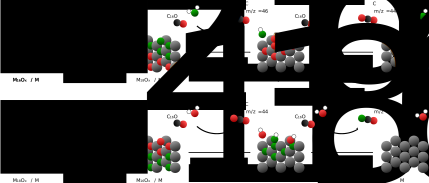
\includegraphics[width=1\textwidth]{04_Oxygen/fig/diagram_O_stripping_with_CO_Pt.png}
	\caption{
		Schematic diagram for exchange and extraction experiments: \textbf{(A)}, An electrode with an unlabeled oxide layer (\ch{M^{16}O}, prepared by oxidation in \ch{H2^{16}O} prior to the experiment) is tested first for exchange (OER) and then extraction (CO oxidation) in labeled electrolyte. \textbf{(B)}, The isotopes are reversed, so the initial oxide layer is labeled and the electrolyte is not labeled.
	}
	\label{fig:Pt_extraction_diagram}
\end{figure}

After many ``negative'' initial results in lattice oxygen evolution experiments (mostly by the less-sensitive procedure A), and ISS not always being available or easy to probe the surface isotopic composition, I wanted a way to check that the desired oxygen isotope had indeed been incorporated into the electrode as lattice oxygen (i.e., did not exchange away spontaneously), ideally without taking the electrode out of the EC-MS setup. 

One clever method of doing so is presented in ref. \citen{Willsau1985}: They oxidize water in un-labeled electrolyte on a Pt film sputtered on a DEMS membrane and oxidized in labeled electrolyte, without observing an isotope signal. Then, to prove the \ch{^{18}O} had indeed been incorporated in the film, they quickly reduce the film, expelling it as \ch{H2^{18}O}, and then jump back to OER potentials. They see a transient m/z=34 signal, which they attribute to oxidation of this liberated \ch{H2^{18}O}. However, they only show the m/z=34 signal and not the m/z=32 signal and they do not show a control experiment. I tried the same experiment without seeing an isotope signal, but this is likely due to the geometry of the setup: whereas in DEMS, constant solvent evaporation leads to a non-negligible convective flow of \ch{H2O} towards the membrane, and thus towards the catalyst when it is sputtered on the DEMS membrane, in our EC-MS setup the electrode surface is separated from the membrane by 100 $\mu$m of still electrolyte, and so the expelled \ch{H2^{18}O} is lost to diffusion in the working volume faster than the electrode potential can be jumped back up to oxidize it. So I had to think of another way.

To prove, in EC-MS, that there was oxygen of a certain isotope in the electrode, I needed to evolve it directly as a gas. If OER did not release lattice oxygen in the evolved \ch{O2}, this meant another reaction involving oxygen and a gaseous product had to be used. I decided to try \ch{CO} oxidation, which we had already used as a model reaction to characterize the EC-MS system (Subsection \ref{subsec:examples}). 

The idea of the experiment is diagrammed in Figure \ref{fig:Pt_extraction_diagram}. It can be done either to prove the existence of a \ch{^{16}O} oxide layer in the presence of \ch{H2^{18}O} electrolyte (Procedure A, Figure \ref{fig:Pt_extraction_diagram}a), or vice versa (Procedure B, Figure \ref{fig:Pt_extraction_diagram}b). Here, I describe it for Procedure A. Data from the corresponding actual experiment is shown in Figure \ref{fig:Pt_extraction_raw}a. The procedure, and results, are as follows:


\begin{figure}[t]
	\centering
	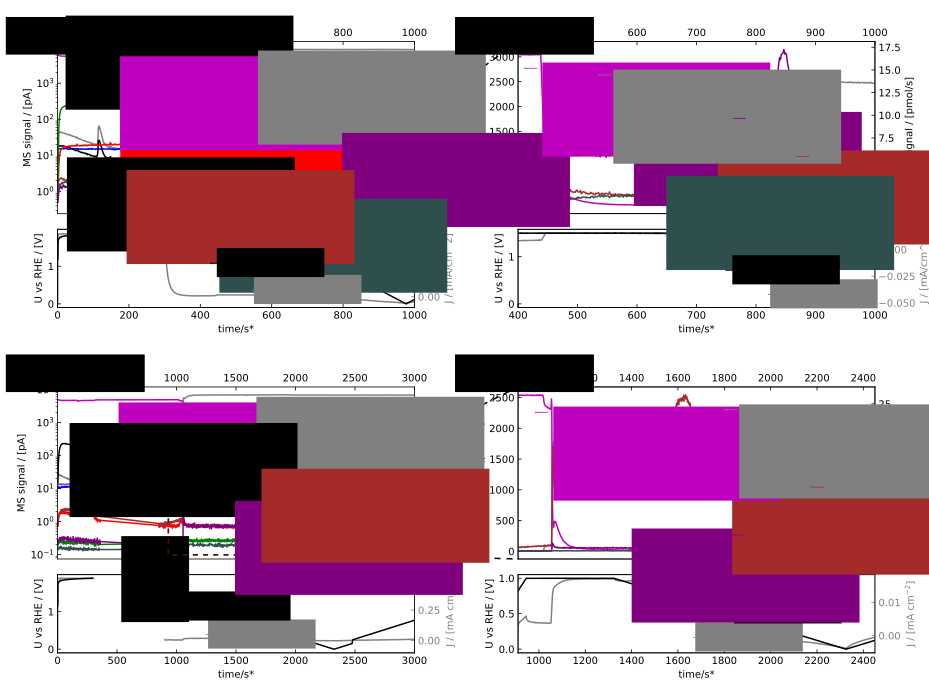
\includegraphics[width=1\textwidth]{04_Oxygen/fig/O_stripping_Pt_raw.png}
	\caption{
		Sequential exchange (OER) and extraction (CO oxidation) experiments on Pt. \textbf{(a)} and \textbf{(b)}, Procedure A of Figure \ref{fig:Pt_extraction_diagram}: Pt with a \ch{Pt^{16}O} layer in labeled electrolyte (0.1 M \ch{HClO4} in 97\% \ch{H2^{18}O}). (a) shows all raw mass signals on a log scale, while (b) shows the calibrated signals for \ch{CO2} on a linear scale during the extraction experiment. The \ch{CO2} signals are on the right y-axis and carrier gas signals are plotted on the left y-axis to show when the switch from \ch{He} to \ch{CO} occurs.
		\textbf{(c)} and \textbf{(d)}, Procedure B of Figure \ref{fig:Pt_extraction_diagram}.
	}
	\label{fig:Pt_extraction_raw}
\end{figure}

\begin{itemize}
\item A metallic polycrystalline \ch{Pt} electrode is oxidized at 100 $\mu$A for ten minutes in un-labeled electrolyte (0.1 M \ch{HClO4} in 99.8\% \ch{H2^{16}O}). Most of the current goes to OER, but some goes to the formation of a \ch{Pt^{16}O} surface layer. The resulting electrode is the starting point in Figure \ref{fig:Pt_extraction_diagram}.

\item This electrode is then placed in the setup with labeled electrolyte (0.1 M \ch{HClO4} in 97\% \ch{H2^{18}O}), and again oxidized at 100 $\mu$A. Simultaneously with OER, we expect that the oxide layer thickens with \ch{Pt^{18}O} at the surface and a ``burried'' layer of \ch{Pt^{16}O}. An ISS depth profile confirming this would be interesting but we haven't gotten around to it yet. 

\item After that, the potential is lowered to a ``resting potential'', here 1.4 V vs RHE, where water is no longer oxidized but the \ch{PtO} layers are not reduced. We dose natural \ch{CO} (99.8\% \ch{C^{16}O}) at this potential. There is relatively little \ch{CO} oxidation current since the \ch{PtO} surface is a much worse catalyst for electrochemical \ch{CO} oxidation than is metalic Pt (see Subsection \ref{subsec:examples}). Most of the CO that is oxidized becomes \ch{C^{16}O^{18}O} (m/z=46) with the \ch{^{18}O} from the electrolyte and the \ch{^{16}O} oxygen atom originating in the \ch{CO} reactant. Some \ch{C^{16}O2} (m/z=44) is present due to the impurity of the electrolyte, and some \ch{C^{18}O2} (m/z=48) is formed by homogeneous oxygen exchange between \ch{C^{16}O^{18}O} and \ch{H2^{18}O} (see Subsection \ref{subsec:isotope_CO2}).

\item Finally, the potential is gradually lowered (here at 5 mV/s). As the surface oxide layer reduces, there is an increase in \ch{CO} oxidation activity. The increase is transient, however, because shortly after the metallic surface is formed, the potential becomes too low to adsorb \ch{$*$OH}, a necessary step in the reaciton. During this transient increase in activity, the buried \ch{^{16}O} isotope is reduced out via \ch{$*$ ^{16}OH}, some of which reacts with \ch{C^{16}O} to form \ch{C^{16}O2}, giving the isotope signal.
\end{itemize}

Figure \ref{fig:Pt_extraction_raw}b shows a zoom-in on the \ch{CO2} isotopic signals during the introduction of \ch{CO} and the reduction of the surface. The \ch{CO2} signals are plotted on the right y-axis, and the carrier gas signals (\ch{He} and \ch{CO}) are plotted on the left y-axis to show exactly when \ch{CO} is dosed. The transient \ch{C^{16}O2} and \ch{C^{16}O^{18}O} signals at the moment that CO is introduced originate within the mass spectrometer (see Subsection \ref{subsec:vacuum_transport}). The ``isotope signal'' is the  \ch{C^{16}O2} transient that starts at $\approx$850 s, right as the reductive wave in the electrode current, as expected for the extraction of a buried labeled oxide layer. 

The same procedure as described above can also be carried out with the isotopes reversed, as shown in Procedure B of Figure \ref{fig:Pt_extraction_diagram}. The result of this experiment is shown in Figures \ref{fig:Pt_extraction_raw}c and d. There are a couple small differences in the procedure: (1) the measurement was stopped and the sample was at OCP for a while between the OER period (exchange experiment) and the CO oxidation period (extraction experiment), (2) the resting potential was 1.0 V vs RHE, leading to a higher steady-state CO oxidation current than at 1.4 V vs RHE, and (3) the potential was scanned at 1 mV/s rather than 5 mV/s. Nonetheless, the results are the same: a transient isotope signal (here for \ch{C^{16}O^{18}O} comes together with the transient increase in overall \ch{CO} oxidation activity as the oxide layer is reduced. A control experiment was also done (\ch{Pt^{16}O} in \ch{H2^{16}O}) which showed no change in the m/z=46 to m/z=44 ratio.

\begin{figure}[t]
	\centering
	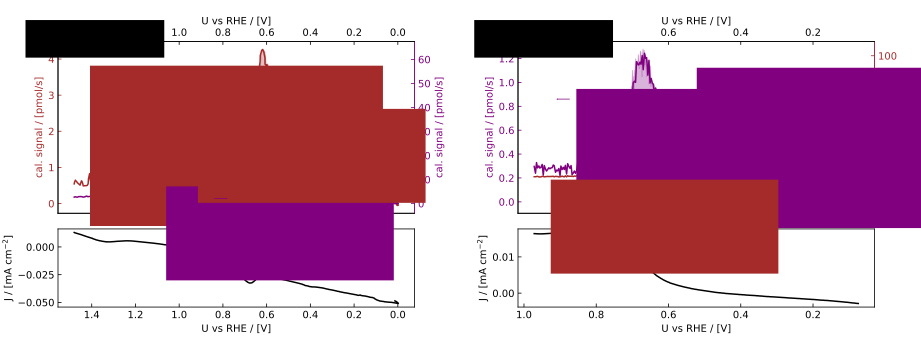
\includegraphics[width=1\textwidth]{04_Oxygen/fig/O_stripping_Pt_extraction.png}
	\caption{
		Analysis of experiments using \ch{CO} oxidation to extract lattice oxygen from a labeled \ch{PtO} layer. In both cases data are plotted against potential. The \ch{CO2} with the labeled oxygen is plotted against the left y-axis and the \ch{CO2} without the label is plotted against the right y-axis. The axes are scaled according to the expected ratio without labeled oxygen from the lattice. \textbf{(a)} Pt with a \ch{Pt^{16}O} layer in labeled electrolyte (0.1 M \ch{HClO4} in 97\% \ch{H2^{18}O}). \textbf{(b)} Pt with a \ch{Pt^{18}O} layer in un-labeled electrolyte (0.1 M \ch{HClO4} in 99.8\% \ch{H2^{16}O}).
	}
	\label{fig:Pt_extraction}
\end{figure}

Figure \ref{fig:Pt_extraction} shows a quantitative analysis of the experiments described above. Here, two axes are used, scaled according to the expected isotopic ratio. For the experiment with \ch{Pt^{16}O} in \ch{H2^{18}O} (Figure \ref{fig:Pt_extraction_raw}a and b, Figure \ref{fig:Pt_extraction}a) this is calculated from the \ch{^{16}O^{18}O} to \ch{^{18}O2} ratio during the OER measurement. This ratio, by the binomial distribution, is
\begin{equation}
r = \frac{\dot{n}_{\ch{^{16}O^{18}O}}}{\dot{n}_{\ch{^{18}O2}}} = \frac{2(x)(1-x)}{(1-x)^2} = \frac{2x}{1-x}\,,\label{eq:r_from_x}
\end{equation}
where $x$ is the electrolyte impurity, i.e.
\begin{equation}
x = \frac{c_{\ch{H2^{16}O}}}{c_{\ch{H2^{16}O}} + c_{\ch{H2^{18}O}}}\,.
\end{equation}
Since the \ch{CO2} (initially) has one oxygen which is \ch{^{16}O} 99.8\% of the time, and only one oxygen from the electrolyte, the expected ratio of \ch{C^{16}O2} to \ch{C^{16}O^{18}O} is $x$. Solving Equation \ref{eq:r_from_x} for $x$ in terms of $r$, which is measured, gives
\begin{equation}
x = \frac{r}{2+r}\,.
\end{equation}
For the experiment with \ch{Pt^{18}O} in \ch{H2^{16}O} (Figure \ref{fig:Pt_extraction_raw}c and d, Figure \ref{fig:Pt_extraction}a), the expected \ch{CO2} is natural \ch{CO2}, and so the ratio is simply determined by measuring the m/z=46 to m/z=44 ratio in natural \ch{CO2}.

In each case the integrated difference between the two curves, thus scaled, is the evolution of labeled lattice oxygen in \ch{CO2}. In both cases, it is about 130 pmol, on the order of 25\% of a monolayer's worth of oxygen (0.196 cm$^2$ of Pt(111) is 490 pmol of surface sites). 

This excellent agreement may, however, be fortuitous. I would expect that the labeling procedure (10 minutes at 100 $\mu$A) would incorporate more than a monolayer's worth of labeled oxygen, and so the small amount of labeled oxygen incorporated into the \ch{CO2} implies a branching, in which some of the reducing oxide reacts with \ch{CO} and some reduces fully, releasing the oxygen as \ch{H2O}. To write it out, for lattice \ch{^{18}O}:
\begin{align}
\ch{$*$ ^{18}O + (H+ + e- ) &-> $*$ ^{18}OH}\Bstrut\\
&\ch{$*$ ^{18}OH + (H+ + e- ) -> H2^{18}O + $*$}\\
&\ch{$*$ ^{18}OH + $*$ C^{16}O -> C^{16}O^{18}O + (H+ + e- ) + 2 $*$}
\end{align}
It is hard to believe that the branching ratios would be exactly the same despite the various differences in the two experimental implementations mentioned above, notably the scan rate. 

Furthermore, 130 pmol is an underestimation, because some of the labeled \ch{CO2} will exchange the labeled oxygen with the electrolyte by the homogeneous reaction going through carbonic acid before it evaporates into the chip, as described in Subsection \ref{subsec:isotope_CO2}. This will have a different effect in the two experiments. When the labeled \ch{CO2} is \ch{C^{16}O2} in \ch{H2^{18}O}-containing electrolyte, the homogeneous exchange reaction is:
\begin{equation}
\ch{C^{16}O2 + H2^{18}O ->[\text{slow}] H2C^{16}O2^{18}O ->[\text{fast}] C^{16}O^{18}O + H2^{16}O}\,.
\end{equation}
In the second step of this reaction, there is a 2/3 chance that the oxygen expelled from carbonic acid is a \ch{^{16}O}, causing the \ch{CO2} to loose its label. (Here, we're making the simplifying omissions of the chance of a \ch{CO2} molecule \textit{picking up} a label from the electrolyte due to the \ch{H2^{16}O} impurity.) In other words, a labeled \ch{CO2} molecule will have to make 1.5 \textit{attempts}, i.e. become carbonic acid 1.5 times on average, before it loses its label. 

 On the other hand, when the labeled \ch{CO2} is \ch{^{16}O^{18}O} in \ch{H2^{16}O}, the homogeneous exchange reaction is
\begin{equation}
\ch{C^{16}O^{18}O + H2^{16}O ->[\text{slow}] H2C^{16}O2^{18}O ->[\text{fast}] C^{16}O2 + H2^{18}O}\,,
\end{equation}
and there is only a 1/3 chance that the \ch{CO2} looses its label. A labeled \ch{CO2} molecule takes 3 attempts on average to lose its label. 

The absolute portion of \ch{CO2} that loses its label to homogeneous scrambling can be estimated by the amount of \ch{C^{18}O2} in Figure \ref{fig:Pt_extraction_raw}b. Here, about 1/5 of the \ch{CO2} comes out as \ch{C^{18}O2}. The majority of this \ch{CO2} started as \ch{C^{16}O^{18}O} and lost the \ch{^{16}O} originally from the CO:
\begin{equation}
\ch{C^{16}O^{18}O + H2^{18}O ->[\text{slow}] H2C^{16}O^{18}O2 ->[\text{fast}] C^{18}O2 + H2^{16}O}\,,
\end{equation}
This takes 3 attempts on average, and so the portion of \ch{C^{16}O2} that with a \ch{^{16}O} from the lattice which loses its label should be about double the steady-state \ch{C^{18}O2} fraction, or about 2/5. Adjusting for this, the total lattice \ch{^{16}O} extracted in the experiment in Figure \ref{fig:Pt_extraction_raw}b is closer to 
\begin{equation}
n^{\ch{C^{16}O2}}_\text{corrected} = n^{\ch{C^{16}O2}}_{\text{measured}} \cdot P(\text{keep label})^{-1} \approx 128 \text{[pmol]} \cdot \left(\frac{3}{5}\right)^{-1} \approx 215 \text{[pmol]}\,,
\end{equation}
which is about 45\% of a monolayer assuming the surface atom density of Pt(111).

Similarly, since it takes 3 attempts for a \ch{CO2} molecule to lose its label in the second experiment, about 1/5 of the labeled \ch{CO2} loses its label to the electrolyte, and the corrected amount of extracted lattice \ch{^{18}O} is
\begin{equation}
n^{\ch{C^{18}O^{16}O}}_\text{corrected} = n^{\ch{C^{18}O^{16}O}}_{\text{measured}} \cdot P(\text{keep label})^{-1} \approx 130 \text{[pmol]} \cdot \left(\frac{4}{5}\right)^{-1} \approx 160 \text{[pmol]}\,,
\end{equation}
or about 33\% of a monolayer assuming the surface atom density of Pt(111).

Despite being quite complex, I think that the results above illustrate that using \ch{CO} as a probe molecule in isotope exchange experiments can be very useful, both as an in-situ proof of labeling when OER does not give an isotope signal, and to investigate the electrochemical reactivity of surface oxygen. I think it would be worth doing systematic experiments of this type, mapping out the effect of the oxide layer thickness, CO dosing potential, and other factors on the isotope signal. This will have to be future work, but I have had time to try similar experiments on a few other materials, including the \ch{Ru} foam material described in Subsection \ref{subsec:Ru_foam}.

\begin{figure}[t]
	\centering
	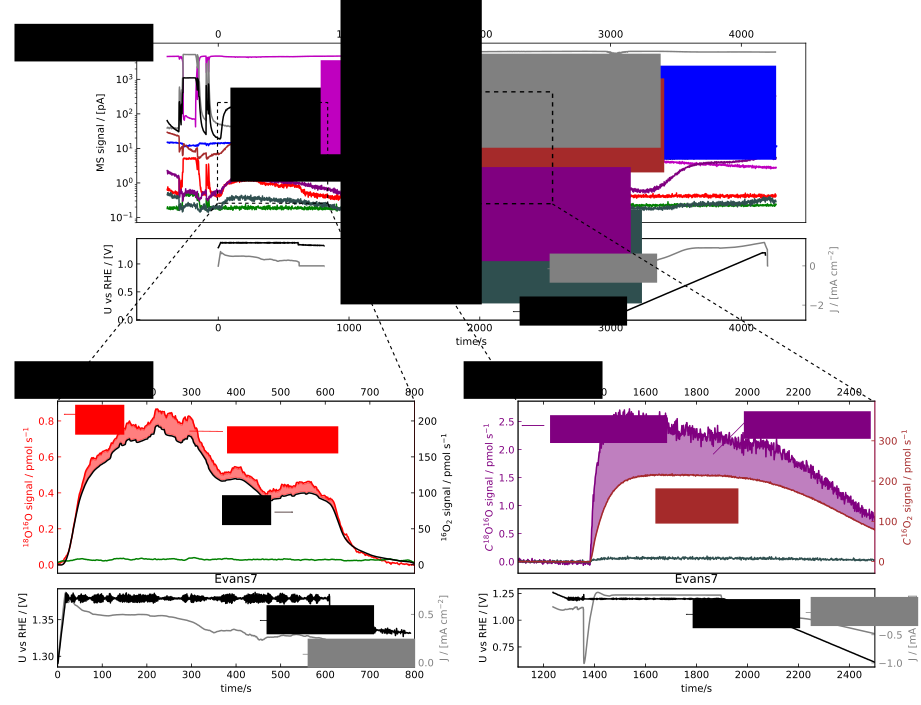
\includegraphics[width=1\textwidth]{04_Oxygen/fig/Evans_exchange_extraction.png}
	\caption{Sequential exchange (OER) and extraction (CO oxidation) experiments probing lattice oxygen reactivity in labeled Ru foam in un-labeled 0.1 M \ch{HClO4}.  \textbf{(a)}, overview showing raw data for both experiments. \textbf{(b)}, Exchange experiment showing excess \ch{^{18}O} compared to natural \ch{^{16}O^{18}O} to \ch{^{16}O2} ratio. \textbf{(c)}, Extraction experiment showing excess \ch{^{18}O} compared to natural \ch{C^{16}O^{18}O} to \ch{C^{16}O2} ratio.
	}
	\label{fig:Evans_extraction}
\end{figure}

Figure \ref{fig:Evans_extraction}a shows the result of sequential lattice oxidation exchange (OER) and extraction (CO oxidation) experiments on \ch{Ru} foam in un-labeled electrolyte (0.1 M \ch{HClO4} in 99.8\% \ch{H2^{16}O}). Prior to this experiment, the foam was labeled by oxidation at 100 $\mu$A for 10 minutes in labeled electrolyte (0.1 M \ch{HClO4} in 97\% \ch{H2^{18}O}). The exchange experiment was done at constant potential (1.38 V vs RHE) rather than constant current. This was a mistake, as it makes it harder to compare directly to other experiments, e.g. those in \ref{fig:EC_Ru}. The current is quite noisy, which can likely be attributed to bubbles (see the discussion around Equation \ref{eq:limiting} above). However, the geometric current density (0.2-0.5 mA/cm$^2$), and thus the total amount of oxygen, are not far from that in Figure \ref{fig:EC_Ru} (0.5 mA/cm$^2$). Thus, it is significant that the amount of excess \ch{^{16}O^{18}O} compared to that expected according to the natural isotopic ratio in Figure \ref{fig:Evans_extraction}b, 26 pmol, is much less than that in Figure \ref{fig:EC_Ru}d, 185 pmol. This difference can attributed to the labeling procedure. Whereas the potential of the Ru foam tested in \ref{fig:EC_Ru}d was cycled in labeled electrolyte before testing in non-labeled electrolyte, the Ru foam tested in Figure \ref{fig:Evans_extraction} was only oxidized at 0.5 mA/cm$^2$ geometric current density for 10 minutes in labeled electrolyte. Apparently, potential cycling either is more effective at incorporating oxygen in a metallic foam than simple oxidation, or the surface oxide layer that potential cycling forms is less stable and releases more of the incorporated \ch{O} during OER.

After the exchange experiment and a brief period at OCP, the electrode potential is brought to 1.23 V vs RHE, and CO is dosed while the potential is held constant. An adsorption transient is seen as a brief ($\approx$ 10 s) cathodic current, which is followed by a steady anodic current and \ch{CO2} production. Compared to the natural isotopic ratio (measured with \ch{CO2} as the carrier gas), there is a clear excess of \ch{C^{16}O^{18}O} (m/z=34) in the evolved \ch{CO2}, indicating that lattice oxygen is being used to oxidize some of the \ch{CO}. This is unlike the experiment on \ch{Pt} (Figure \ref{fig:Pt_extraction}), where the isotope signal did not come until the oxide layer was reduced. This might indicate that an oxidized layer on \ch{Ru} can react with \ch{CO} in a way that an oxidized layer on Pt can not. However, it may just be an artifact of the much higher surface area of the Ru foam, which has a roughness factor on the order of 2000 (see Subsection \ref{subsec:Ru_foam}). A control experiment with Ru foam that had not seen labeled electrolyte did not show an isotope signal during \ch{CO} oxidation.

Reducing the surface of the \ch{Ru} did not extract more \ch{^{18}O} - in fact, the \ch{C^{16}O^{18}O} to \ch{C^{16}O2} ratio decreases when the potential is lowered below 1 V vs RHE, as does the overall CO oxidation activity. This ratio, however, increases again when the sample is brought to anodic potentials again, indicating that one cathodic sweep down to 0 V vs RHE was not enough to reduce all of the \ch{^{18}O} out of the sample, or that not all the \ch{H2^{18}O} formed escaped the porous structure of the sample. While there is great potential for using this type of experiment to explore the surface electrochemistry of Ru, for now it has served its purpose: Since much more \ch{^{18}O} could be extracted from the electrode by \ch{CO} oxidation than was exchanged during OER, it proves that there is much electrochemically accessible oxygen which is not lost from the catalyst during oxygen evolution. In other words, it not only confirms that lattice oxygen exchange is not a primary OER mechanism on ruthenium, but also indicates that, at least at very low TOF, there are surface oxygen species which are spectators to OER.

That concludes this Section on lattice oxygen reactivity. However, the best experiments have been saved for the next Section, because as we got better at doing isotope-labeling studies, we also started to relate lattice oxygen evolution to metal dissolution.

%As a final note to this Section on lattice oxygen reactivity, before it is related to stability in the next Section, I would like to point out the participation of lattice oxygen in one last reaction: the oxidation of adventitious carbon.



